\documentclass[aspectratio=169]{beamer}
\usepackage{graphicx}
\usepackage[italian]{babel}
\usepackage{hyperref}
\usepackage{tikz}

\usetheme[progressbar=frametitle]{metropolis}
\title{Quantum Approaches to Sentiment Analysis}
\author{\emph{Candidate}: Mario Bifulco}
\date{\emph{Supervisor}: Luca Roversi}
\institute{University of Turin}

\begin{document}
\setbeamertemplate{section in toc}[sections numbered]

\begin{frame}
    \titlepage
\end{frame}

\section{Quantum Support Vector Machine for Sentiment Analysis}

\begin{frame}
    \frametitle{Why use non-classical architectures?}

    \begin{columns}
        \begin{column}{0.3\textwidth}
            \begin{itemize}
                \item Ampliamento dei problemi trattabili
                \item Reversibilità delle procedure di calcolo
            \end{itemize}
        \end{column}
        \begin{column}{0.7\textwidth}
            \begin{flushright}
                \includegraphics[height=0.9\textheight]{bqp_complexity.png}
            \end{flushright}
        \end{column}
    \end{columns}

\end{frame}

\begin{frame}
    \frametitle{Why Adiabatic quantum computing?}

    \begin{columns}
        \begin{column}{0.6\textwidth}
            \begin{flushleft}
                \includegraphics[width=\textwidth]{q_anneal.png}
            \end{flushleft}
        \end{column}
        \begin{column}{0.4\textwidth}
            \begin{itemize}
                \item Ricerca di minimi globali
                \item Effetto tunnel per superare minimi locali
            \end{itemize}
        \end{column}
    \end{columns}

\end{frame}

\begin{frame}
    \frametitle{Why Support Vector Machine?}

    \begin{itemize}
        \item Problema di ottimizzazione quadratico
        \item Formulazione naturale in CSP
        \item Classificazione binaria di punti su uno spazio multidimensionale
    \end{itemize}

\end{frame}

\begin{frame}
    \frametitle{Empirical comparison}

    Confronto sul task di Sentiment Analysis tramite il dataset TweetEval

    \begin{itemize}
        \item Solver classico (CPU)
        \item Solver ibrido (QPU + CPU)
        \item Architetture Transformer (GPU)
    \end{itemize}

\end{frame}

\begin{frame}
    \frametitle{Qualitative analysis}

    Risultati medi su 10 esecuzioni:

    \begin{table}
        \centering
        \begin{tabular}{c|c|c|c}
            & CPLEX & D-Wave & RoBERTa \\ \hline
            F1-Score (\%) & 76.9 & 76.1 & 94.3 \\ \hline
            Train time (s) & 267.4 & 327.8\footnote{Solo 40s vengono impiegati dal solver per risolvere il problema} & /\footnote{È stato utilizzato il modello pre-trained sul dataset TweetEval} \\ \hline
            Eval time (s) & 2.2 & 33.9 & 136.8
        \end{tabular}
    \end{table}

\end{frame}

\section{Balancing QPU and CPU \\execution time}

\begin{frame}
    \frametitle{Usage of QPU}

    \begin{columns}
        \begin{column}{0.4\textwidth}
            \begin{itemize}
                \item Solo lo 0.08\% del tempo è speso sulla QPU
                \item Il boost prestazionale deriva dal quantum annealing
                \item È possibile trasformare il problema per risolverlo nativamente in QPU?
            \end{itemize}
        \end{column}
        \begin{column}{0.6\textwidth}
            \begin{flushright}
                \includegraphics[height=0.8\textheight]{piechart.png}
            \end{flushright}
        \end{column}
    \end{columns}

\end{frame}

\begin{frame}
    \frametitle{The problem of the minor embedding algorithm}

    \begin{columns}
        \begin{column}{0.4\textwidth}
            \begin{flushleft}
                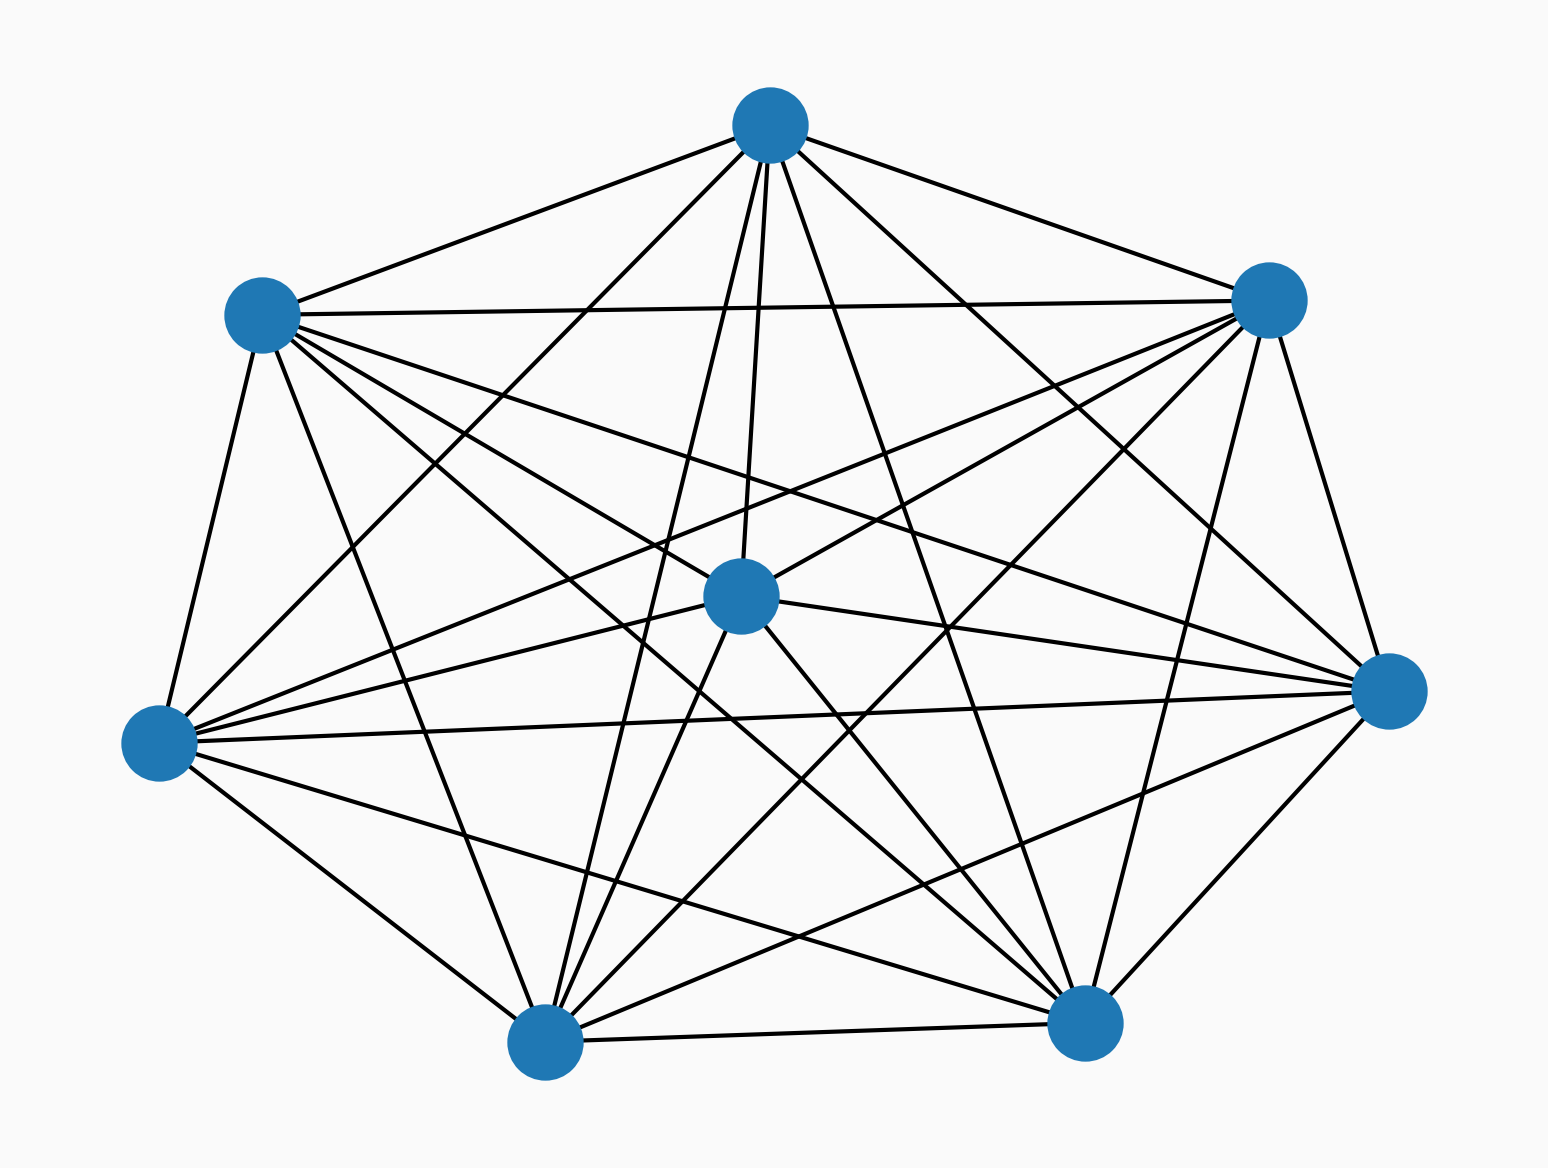
\includegraphics[width=\textwidth]{source.png}
            \end{flushleft}
        \end{column}
        \begin{column}{0.1\textwidth}
            \LARGE
            $\Longrightarrow$
        \end{column}
        \begin{column}{0.4\textwidth}
            \begin{flushright}
                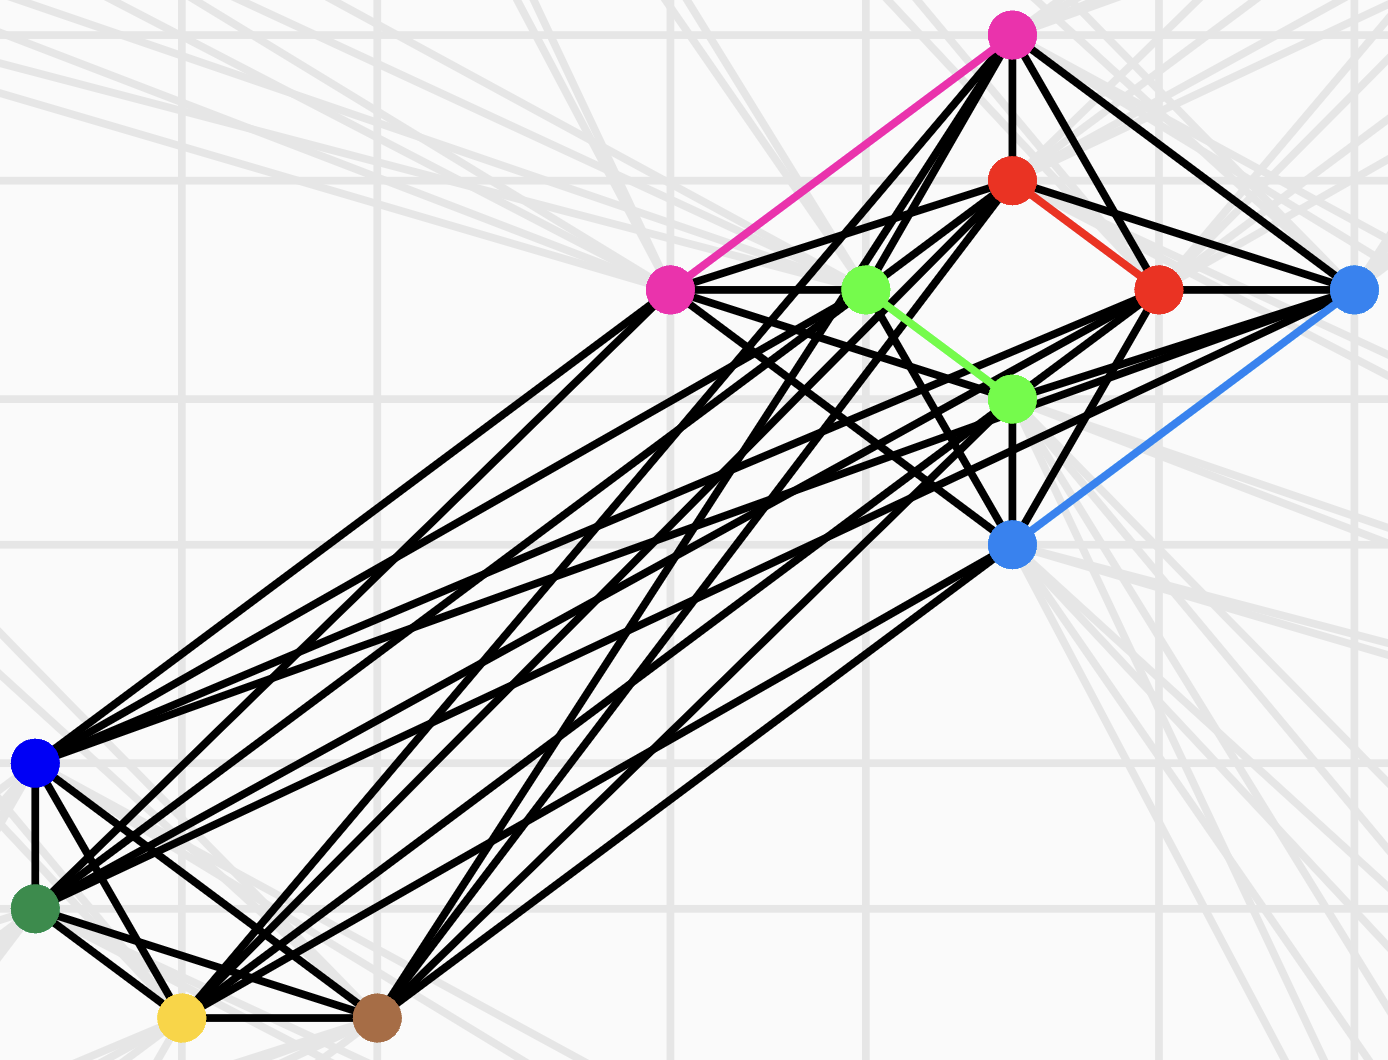
\includegraphics[width=\textwidth]{target.png}
            \end{flushright}
        \end{column}
    \end{columns}

    \begin{center}
        Mapping del grafo che descrive il problema verso il grafo Pegasus.        
    \end{center}

\end{frame}

\begin{frame}
    \frametitle{Embedding Search Times}

    \begin{table}
        \centering
        \begin{tabular}{c|c|c}
            Problem Nodes & Embedding Nodes & Avg Time (s) \\ \hline
            4 & 4 & 0.2 \\
            8 & 13 & 0.3 \\
            16 & 40 & 0.6 \\
            32 & 138 & 6.1 \\
            64 & 526 & 53.4 \\
            128 & 2117 & 434.2 \\
        \end{tabular}
    \end{table}

    \begin{center}
        La QPU Pegasus ha un numero di 5627 QuBit
    \end{center}

\end{frame}

\section{Developing an hybrid solver}

\begin{frame}
    \frametitle{Algebric decomposition of QUBO problems}

    

\end{frame}

\begin{frame}
    \frametitle{Results}

    

\end{frame}

\begin{frame}
    \frametitle{Future works}

    

\end{frame}

\end{document}